\section{Design Patterns in der Software-Entwicklung}

Entwurfsmuster definieren gängige Lösungsblaupausen für häufig auftretende Probleme in Software-Entwicklung, vor allem in der Design-Phase der Architektur des Software-Systems
als auch während der konkreten Implementierung. Jedoch sind diese als Schablone zu verstehen, die für den jeweiligen Einsatzfall angepasst werden müssen.
Ein Werk, dass das Verständnis von Design Patterns für das objektorientierte Programmieren maßgeblich geprägt, ist das von Gamma et al. verfasste Arbeit "Design Patterns: Elements of Reusable Object-Oriented Software".
In diesem wird ein Katalog von 23 Entwurfsmustern definiert, welche in drei Kategorien aufgeteilt. Dieser Katalog wird von Software-Entwicklern als "Gang of Four" Entwurfsmuster bezeichnet. Gamma et al. definieren folgende Elemente für die Identifikation eines Entwurfsmusters:\cite[S. 3]{gamma1994design}

\begin{itemize}
    \item \textbf{Pattern Name}: Der Name des Entwurfsmusters beschreibt in wenigen Worten, welches das zu lösende Problem, die Lösung und welche Folgen dessen Einsatz mit sich bringt. Durch die Einführung eines Bezeichners wird eine Schicht der Abstraktion hinzugefügt, welches das Verständnis und Dokumentation des Design Patterns vereinfacht.
    \item \textbf{Problem}: Das Problem beschreibt, wo das Entwurfsmuster angewendet werden soll. Dabei kann es sich um ein konkretes Entwurfsproblem, Klassen- oder Objektstrukturen oder eine Liste von Bedingungen darstellen, die zu erfüllen sind.
    \item \textbf{Solution}: Das Lösungselement beschreibt die Beziehungen, Verantwortlichkeiten und Zusammenarbeit der einzelnen Elemente, die die Struktur des Design Patterns definieren. Dabei werden diese Elemente in Objekte und Klassen, die die Grundbausteine der objektorientierten Programmierung repräsentieren, aufgeteilt und deren Interaktionen miteinander stellen die Verantwortlichkeiten und Beziehungen dar.
    \item \textbf{Consequences}: Die Folgen diskutieren, wie der Einsatz des betrachteten Entwurfsmusters sich auf das Software-System einwirkt und welche Vor- und Nachteile dadurch resultieren. Diese beeinflussen unter anderem die Zeit- und Speicherkomplexität, Erweiterbarkeit, Flexibilität und Portabilität des Software-Systems.
\end{itemize}

Im Kontext dieser Arbeit werden zu klassifizierende Strukturen, die potenziell einem Design Pattern zugeordnet werden können, als Mikroarchitekturen bezeichnet, die aus einer Menge von interagierenden Komponenten bestehen, denen je eine Rolle zugewiesen wird. Die jeweilige Rolle beschreibt, welche Funktionalität und Verantwortung diese im Kontext der Mikroarchitektur übernimmt und wie diese mit anderen Komponenten interagiert.
Als Komponenten mit Rollen werden hier konkrete bzw\. abstrakte Klassen oder Schnittstellen definiert, die erforderte Rolle im Rahmen der Mikroarchitektur erfüllen.

In weiteren Verlauf dieser Sektion werden die drei erwähnten Entwurfsmusterkategorien erläutert und zu dem werden im Kontext dieser Arbeit betrachte spezifische Design Pattern genauer betrachtet.

\newpage

\section{Design Pattern Katalog}

\subsection{Creational Design Patterns}

Die Kategorie der Creational Design Patterns oder Erzeugungsentwurfsmuster beschäftigt sich mit der Abstraktion des Prozesses der Initialisierung\cite[S. 81]{gamma1994design}. Entwurfsmuster dieser Kategorie fokussieren sich auf die Unabhängigkeit wie Objekte erstellt, zusammengesetzt und repräsentiert werden.
Die Entwurfsmuster dieser Kategorie mit Fokus auf Klassen nutzen den Mechanismus der Vererbung, um zu beeinflussen, wie Komponenten instantiiert werden, während dahingegen Design Patterns mit einem Fokus auf Objekten die Instantiierung auf andere Objekte delegieren.
Creational Design Patterns werden dann bedeutend, wenn mit steigender Komplexität des Software-Systems sich von Vererbung distanziert wird und die Komposition aus einzelnen definierten Objekt mehr an Bedeutung gewinnt\cite[S. 81]{gamma1994design}. Dabei wird das Verhalten einer Komponente auf eine Menge von einzelnen kleinere Objekten delegiert und durch Zusammensetzung innerhalb der Komponente und deren Interaktion das erwünschte Verhalten erzeugt.
Dadruch wird die Instantiierung von Software-Komponenten komplexer, da die Instantiierung von mehreren Objekten koordiniert werden muss. Creational Design Patterns liefern hierbei Hilfestellung, weil die exakte Komposition der konkreten Objekte, die Teil der zu instantiierenden Komponente sind, und der exakte Prozess der Instantiierung im Inneren des Entwurfsmusters verborgen werden. Nach außen hin sind dahingegen nur die Schnittstellen sichtbar, die die Komponente zur Verfügung stellt, während dessen interene Logik die Ausführung auf andere Objekte delegiert.
Im Kontext dieser Arbeit werden folgende Entwurfsmuster aus der Kategorie der Creational Design Patterns betrachtet:

\subsubsection{Singleton}

\begin{figure}[h]
    \centering
    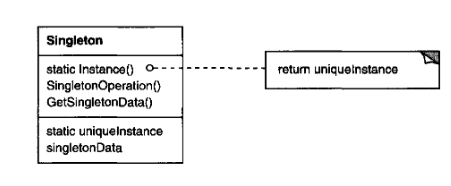
\includegraphics{figures/singleton.png}
    \caption{UML-Diagramm für Singleton}
    \label{fig:singleton}
\end{figure}

Die Abbildung~\ref{fig:singleton} zeigt den strukturellen Aufbau eines Singletons~\cite[S. 127]{gamma1994design}.
Dabei kann dieser nach Gamma et al. wie folgt beschrieben werden:

\begin{description}
    \item[Problem] \hfill \\
    \begin{itemize}
        \item Exakt eine Instanz der Klasse zur selben Zeit verfügbar; Zugreifbar zu Klienten durch bekannten Zugangspunkt
        \item Einzige Instanz erweiterbar durch Vererbung; Nutzbarkeit der Subklasse ohne Veränderung des Quellcodes auf Klientenseite
    \end{itemize}
    \item[Solution] \hfill
    \begin{itemize}
        \item   Zugriff auf Singleton-Instanz durch Instance-Operation
    \end{itemize}
    \item[Roles] \hfill \\
    \begin{description}
        \item[Singleton] \hfill \\
        \begin{itemize}
            \item Definiert eine Instance-Operation für Zugriff auf einzige Instanz
            \item Mögliche selbstsändige Instanziierung
        \end{itemize}
    \end{description}
    \item[Consequences]  \hfill 
    \begin{itemize}
        \item Kontrollierter Zugriff auf Instanz
        \item Mögliche Verfeinerung der Operationen und Repräsentation durch Vererbung
        \item Nachträgliche Änderung der Anzahl der Instanzen 
    \end{itemize}
\end{description}

\subsubsection{Factory Method}

\begin{figure}[h]
    \centering
    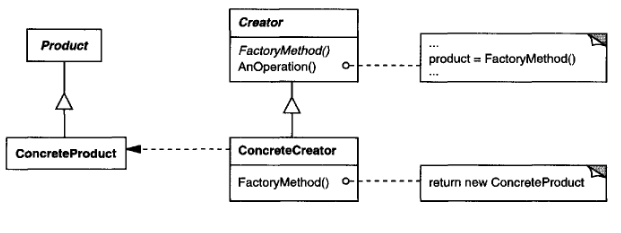
\includegraphics[scale=0.8]{figures/factory.png}
    \caption{UML-Diagramm für Factory Method}
    \label{fig:factory}
\end{figure}

Abbildung~\ref{fig:factory} beschreibt exemplarisch die Struktur einer Factory Method~\cite[S. 108]{gamma1994design}.
Diese wird nach Gamma et al. auf folgende Art und Weise beschrieben:

\begin{description}
    \item[Problem] \hfill 
    \begin{itemize}
        \item Eine Klasse kann die Klasse der Objekte, die es instantiiert, im Voraus nicht erahnen
        \item Eine Klasse verlangt, dass ihre Unterklassen die von ihr erstellten Objekte spezifizieren
        \item Klassen delegieren die Instantiierung von Objekten an Helferklassen
    \end{itemize}

    \item[Role] \hfill
    \begin{description}
        \item[Product] \hfill
        \begin{itemize}
            \item definiert die Schnittstelle der Objekte, die die Factory-Methode erzeugt
        \end{itemize}
        \item[ConcreteProduct] \hfill
        \begin{itemize}
            \item implementiert die Schnittstelle Product
        \end{itemize}
        \item[Creator] \hfill 
        \begin{itemize}
            \item deklariert die Factory-Methode, die ein Objekt vom Typ Product zurückgibt
            \item kann auch eine Standardimplementierung der Factory-Methode definieren, die die ein Standard ConcreteProduct-Objekt zurückgibt
            \item kann die Factory-Methode aufrufen, um ein Product-Objekt zu erzeugen
        \end{itemize}
        \item[ConcreteCreator] \hfill
        \begin{itemize}
            \item überschreibt die Factory-Methode, um eine Instanz eines ConcreteProduct zurückzugeben
        \end{itemize}
    \end{description}

    \item[Consequences] \hfill
    \begin{itemize}
        \item Eliminierung der Bindung an applikationsspezifische Klassen; Interaktion durch Product-Schnittstelle
        \item Flexibilität bei der Instanziierung von Objekten.
    \end{itemize}

\end{description}


%%TODO: Add concrete design patterns
\subsubsection{Structural Design Patterns}

Structural Design Patterns oder Strukturentwurfsmuster fokussieren sich darauf, wie einzelne Klassen und Objekte zusammengesetzt werden können, um größere Strukturen zu erzeugen\cite[S. 137]{gamma1994design}.
Entwurfsmuster dieser Kategorie sind vorteilhaft, wenn unabhängig voneinander entwickelte Klassen oder Objekte aus verschiedenen Bibliotheken oder Frameworks miteinander interagieren müssen.
Anstatt konkrete Implementierung und Schnittstellen zu nutzen, bedienen sich Structural Design Patterns der Komposition aus Objekten, um neue Funktionalitäten zur Verfügung zu stellen\cite[S. 137]{gamma1994design}.
Die dadurch gewonnene Flexibilität ermöglicht das Ändern der Zusammensetzung des Objektes dynamisch zu der Laufzeit, welches mit statischer Komposition durch Klassen nicht möglich ist.\cite[S. 137]{gamma1994design}.
Im Kontext dieser Arbeit werden folgende Entwurfsmuster aus der Kategorie der Structural Design Patterns betrachtet:

\subsubsection{Adapter}

\begin{figure}[h]
    \centering
    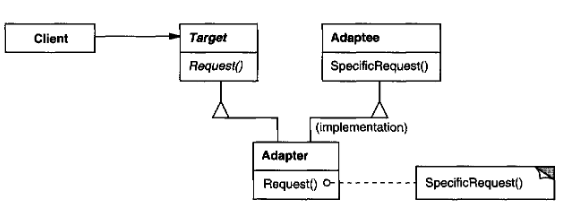
\includegraphics[scale=0.75]{figures/adapter.png}
    \caption{UML-Diagramm für Adapter}
    \label{fig:adapter}
\end{figure}

Abbildung~\ref{fig:adapter} zeigt die Struktur des Adapter-Entwurfsmusters. 
Dabei wird ein Adapter nach Gamma et al. wie gefolgt beschrieben~\cite[S. 141]{gamma1994design}:


.\begin{description}
    \item[Problem] \hfill
    \begin{itemize}
        \item Eine existierende Klasse soll genutzt werden; die Schnittstelle der Klasse stimmen mit der gebrauchten nicht überein
        \item Recyclebare Klasse, die mit unabhängigen Klassen kooperiert
    \end{itemize}
    \item[Roles] \hfill
    \begin{description}
        \item[Target] \hfill
        \begin{itemize}
            \item definiert domain-spezifische Schnittstelle für das Nutzen durch Clients
        \end{itemize}
        \item[Client] \hfill 
        \begin{itemize}
            \item kollaboriert mit Objekten, die Target-Schnittstelle implementieren
        \end{itemize}
        \item[Adaptee] \hfill 
        \begin{itemize}
            \item definiert ein bereits existierende Schnittstelle, worauf Adapter abgepasst wird
        \end{itemize}
        \item[Adapter] \hfill 
        \begin{itemize}
            \item adoptiert die Schnittstelle von Adaptee zu Target-Schnittstelle
        \end{itemize}
    \end{description}
    \item[Consequences] \hfill 
        \begin{itemize}
            \item Adoptierung von Adaptee zu Target-Schnittstelle durch konkrete Adapter-Klasse
            \item Adapter überschreibt Verhalten von Adaptee-Klasse, da Adapter Subklasse von Adaptee 
        \end{itemize}
\end{description}

\pagebreak

\subsubsection{Behavioral Design Patterns}

Behavioral Design Patterns oder Verhaltensentwurfsmuster konzentrieren sich auf Algorithmen und der Zuweisung von Verantwortlichkeiten zwischen Objekten\cite[S. 221]{gamma1994design}.
Dabei wird nicht nur Struktur der Entwurfsmuster betrachtet, sondern auch die Kommunikation und Interaktion der Objekte, die Teil des Entwurfsmusters sind. Charakteristisch für Design Patterns dieser Kategorie ist der Fokus auf Verknüpfung der einzelnen Teilobjekte des Entwurfsmusters,
anstatt des Kontrollflusses, welcher zur Laufzeit schwer nachvollziehbar sein kann~\cite[S. 221]{gamma1994design}.
Im Kontext dieser Arbeit werden folgende Entwurfsmuster aus der Kategorie der Behavioral Design Patterns betrachtet:

\subsubsection{Command}

\begin{figure}[h]
    \centering
    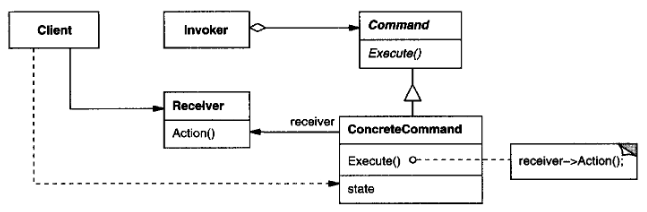
\includegraphics[scale=0.75]{figures/command.png}
    \caption{UML-Diagramm für Command}
    \label{fig:command}
\end{figure}

Abbildung~\ref{fig:command} zeigt die Struktur des Adapter-Entwurfsmusters. 
Dabei wird Command nach Gamma et al. wie gefolgt beschrieben~\cite[S. 236]{gamma1994design}:

\begin{description}
    \item[Problem] \hfill 
    \begin{itemize}
        \item Kapsulierung von Aktion durch parametrisierbare Objekte
        \item Spezifizierung, Abwarten und Ausführung von Aktionen zu verschiedenen Zeiten;
        \item Option für Undo; ausgeführte Aktion wird rückgängig gemacht
    \end{itemize}
    \item[Roles] \hfill
    \begin{description}
        \item[Command] \hfill
        \begin{itemize}
            \item deklariert eine Schnittstelle für das Ausführen von Operationen
        \end{itemize}
        \item[ConcreteCommand] \hfill
        \begin{itemize}
            \item definiert eine Bindung zwischen einem Receiver und einer Aktion
            \item implementiert Execute-Methode durch Ausführen des korrespondierenden Operationen auf Seite von Receiver
        \end{itemize}
        \item[Invoker] \hfill
        \begin{itemize}
            \item initialisiert die Ausführung eines Commands
        \end{itemize}
        \item[Receiver] \hfill
        \begin{itemize}
            \item Empfänger von Commands
            \item Wissen, wie empfangene Commands auszuführen sind  
        \end{itemize}
    \end{description}
    \item[Consequences] \hfill
    \begin{itemize}
        \item Entkoppelung zwischen Objekt, welches Operation initialisiert, und Objekt, das Operation durchführt
        \item Erweiterung von Manipulation von Verhalten von Command-Klassen durch Vererbung
        \item Zusammensetzung von Command-Klassen durch andere Command-Klassen
        \item Erleichtertes Hinzufügen von neuen Command-Klassen
    \end{itemize}
\end{description}

\subsubsection{Observer}

\begin{figure}[h]
    \centering
    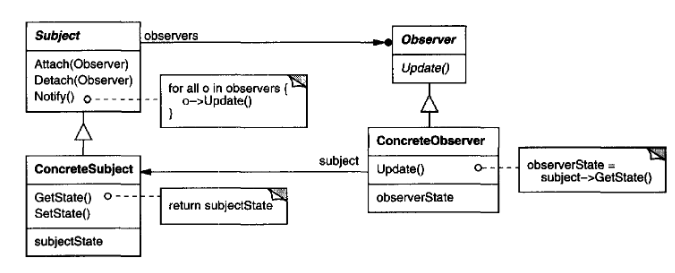
\includegraphics[scale=0.75]{figures/observer.png}
    \caption{UML-Diagramm für Observer}
    \label{fig:observer}
\end{figure}

Die Abbildung~\ref{fig:observer} zeigt den strukturellen Aufbau eines Observers~\cite[S. 293]{gamma1994design}.
Dabei kann dieser nach Gamma et al. wie folgt beschrieben werden:

\begin{description}
    \item[Problem] \hfill 
    \begin{itemize}
        \item Benachrichtigung von Objekten ohne Annahmen über diese
        \item Änderung in einem Objekt erfordert Änderungen in abhängigen Objekten; Kein Wissen wie abhängige Objekte auf Änderung reagieren
    \end{itemize}
    \item[Roles] \hfill
    \begin{description}
        \item[Subject] \hfill 
        \begin{itemize}
            \item Wissen über dessen Observer; beliebige Anzahl an Observern an einem Subject möglich
            \item Schnittstelle für das Hinzufügen und Entfernen von Observern
        \end{itemize}
        \item[Observer] \hfill 
        \begin{itemize}
            \item definiert Schnittstelle für das Reagieren von Änderungen am Subject seitens der abhängigen Objekte
        \end{itemize}
        \item[ConcreteSubject] \hfill 
        \begin{itemize}
            \item implementiert Subject-Schnittstelle
            \item beinhaltet relevanten Zustand von ConcreteObserver-Objekten
            \item Benachrichtigung von dessen Observer-Objekten bei Änderungen am relevanten Zustand
        \end{itemize}
        \item[ConcreteObserver] \hfill 
        \begin{itemize}
            \item hält Referenz zu ConcreteSubject-Objekt
            \item Speichert selbst Zustand; konsistent zu dem von Subject
            \item implementiert Observer-Schnittstelle für das Synchronisieren der Zustände  
        \end{itemize}
    \end{description}
    \item[Consequences]:
    \begin{itemize}
        \item Abstrakte Koppelung zwischen Observer und Subject; Keine Annahmen von Subject über Observer außer Observer-Schnittstelle
        \item Broadcast an Observer; Benachrichtigung aller registrierten Observer
        \item Einspielen von unerwarteten Benachrichtigung 
    \end{itemize}
\end{description}